\documentclass{standalone}
\usepackage{tikz}
\usetikzlibrary{patterns, positioning}

\begin{document}
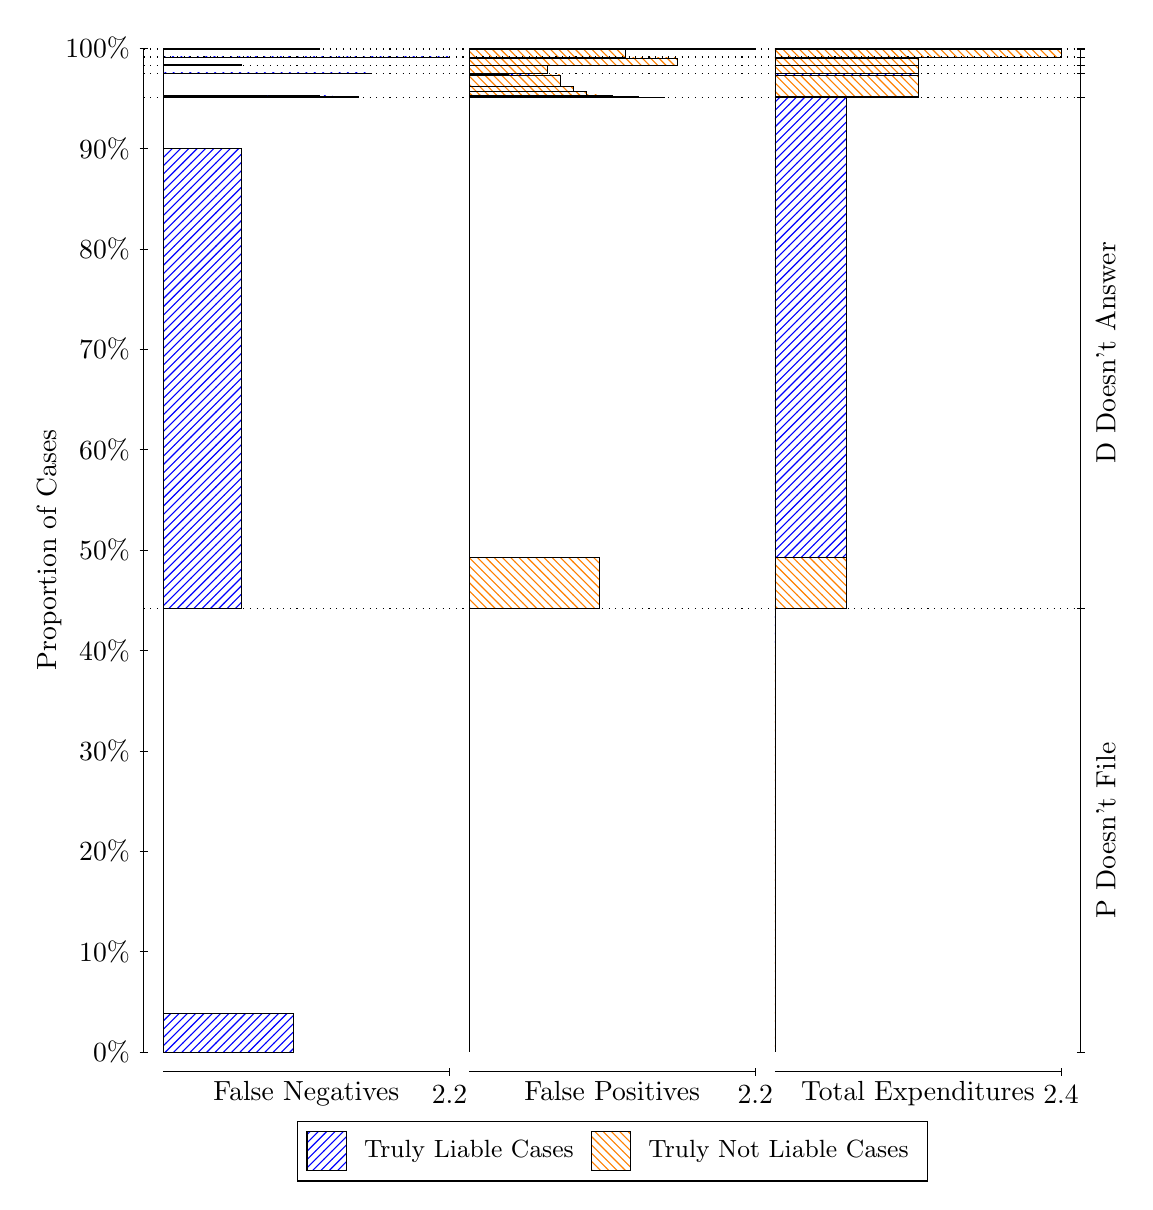
\begin{tikzpicture}
\draw[black, very thin] (1.5,1.75) -- (1.5,14.5);
\node[rotate=90, anchor=center] at (0.3, 8.125) {Proportion of Cases};
\draw[black, very thin] (1.45,1.75) -- (1.55,1.75);
\node[anchor=east] at (1.45, 1.75) {0\%};
\draw[black, very thin] (1.45,3.025) -- (1.55,3.025);
\node[anchor=east] at (1.45, 3.025) {10\%};
\draw[black, very thin] (1.45,4.3) -- (1.55,4.3);
\node[anchor=east] at (1.45, 4.3) {20\%};
\draw[black, very thin] (1.45,5.575) -- (1.55,5.575);
\node[anchor=east] at (1.45, 5.575) {30\%};
\draw[black, very thin] (1.45,6.85) -- (1.55,6.85);
\node[anchor=east] at (1.45, 6.85) {40\%};
\draw[black, very thin] (1.45,8.125) -- (1.55,8.125);
\node[anchor=east] at (1.45, 8.125) {50\%};
\draw[black, very thin] (1.45,9.4) -- (1.55,9.4);
\node[anchor=east] at (1.45, 9.4) {60\%};
\draw[black, very thin] (1.45,10.675) -- (1.55,10.675);
\node[anchor=east] at (1.45, 10.675) {70\%};
\draw[black, very thin] (1.45,11.95) -- (1.55,11.95);
\node[anchor=east] at (1.45, 11.95) {80\%};
\draw[black, very thin] (1.45,13.225) -- (1.55,13.225);
\node[anchor=east] at (1.45, 13.225) {90\%};
\draw[black, very thin] (1.45,14.5) -- (1.55,14.5);
\node[anchor=east] at (1.45, 14.5) {100\%};

\draw[black, very thin] (13.4,1.75) -- (13.4,14.5);
\draw[black, very thin] (13.35,1.75) -- (13.45,1.75);
\node[anchor=west] at (13.35, 1.75) {};
\draw[black, very thin] (13.35,7.3803) -- (13.45,7.3803);
\node[anchor=west] at (13.35, 7.3803) {};
\draw[black, very thin] (13.35,13.875) -- (13.45,13.875);
\node[anchor=west] at (13.35, 13.875) {};
\draw[black, very thin] (13.35,14.182) -- (13.45,14.182);
\node[anchor=west] at (13.35, 14.182) {};
\draw[black, very thin] (13.35,14.279) -- (13.45,14.279);
\node[anchor=west] at (13.35, 14.279) {};
\draw[black, very thin] (13.35,14.386) -- (13.45,14.386);
\node[anchor=west] at (13.35, 14.386) {};
\draw[black, very thin] (13.35,14.488) -- (13.45,14.488);
\node[anchor=west] at (13.35, 14.488) {};
\draw[black, very thin] (13.35,14.5) -- (13.45,14.5);
\node[anchor=west] at (13.35, 14.5) {};

\draw[black, very thin, pattern color=blue, pattern=north east lines] (1.75,1.75) rectangle (3.4015,2.2355);
\draw[black, very thin, pattern color=orange, pattern=north west lines] (1.75,2.2355) rectangle (1.75,7.3803);
\draw[black, very thin, pattern color=blue, pattern=north east lines] (1.75,7.3803) rectangle (2.7409,13.226);
\draw[black, very thin, pattern color=orange, pattern=north west lines] (1.75,13.226) rectangle (1.75,13.875);
\draw[black, very thin, pattern color=blue, pattern=north east lines] (1.75,13.875) rectangle (4.2273,13.886);
\draw[black, very thin, pattern color=blue, pattern=north east lines] (1.75,13.886) rectangle (4.0621,13.89);
\draw[black, very thin, pattern color=blue, pattern=north east lines] (1.75,13.89) rectangle (3.897,13.892);
\draw[black, very thin, pattern color=blue, pattern=north east lines] (1.75,13.892) rectangle (3.7318,13.894);
\draw[black, very thin, pattern color=blue, pattern=north east lines] (1.75,13.894) rectangle (3.5667,13.895);
\draw[black, very thin, pattern color=blue, pattern=north east lines] (1.75,13.895) rectangle (3.4015,13.896);
\draw[black, very thin, pattern color=blue, pattern=north east lines] (1.75,13.896) rectangle (3.2364,13.897);
\draw[black, very thin, pattern color=blue, pattern=north east lines] (1.75,13.897) rectangle (3.0712,13.897);
\draw[black, very thin, pattern color=blue, pattern=north east lines] (1.75,13.897) rectangle (2.9061,13.898);
\draw[black, very thin, pattern color=orange, pattern=north west lines] (1.75,13.898) rectangle (1.75,14.182);
\draw[black, very thin, pattern color=blue, pattern=north east lines] (1.75,14.182) rectangle (4.3924,14.185);
\draw[black, very thin, pattern color=orange, pattern=north west lines] (1.75,14.185) rectangle (1.75,14.279);
\draw[black, very thin, pattern color=blue, pattern=north east lines] (1.75,14.279) rectangle (2.7409,14.291);
\draw[black, very thin, pattern color=orange, pattern=north west lines] (1.75,14.291) rectangle (1.75,14.386);
\draw[black, very thin, pattern color=blue, pattern=north east lines] (1.75,14.386) rectangle (5.3833,14.388);
\draw[black, very thin, pattern color=orange, pattern=north west lines] (1.75,14.388) rectangle (1.75,14.488);
\draw[black, very thin, pattern color=blue, pattern=north east lines] (1.75,14.488) rectangle (3.7318,14.492);
\draw[black, very thin, pattern color=orange, pattern=north west lines] (1.75,14.492) rectangle (1.75,14.5);
\draw[black, very thin, pattern color=orange, pattern=north west lines] (5.6333,1.75) rectangle (5.6333,6.8948);
\draw[black, very thin, pattern color=blue, pattern=north east lines] (5.6333,6.8948) rectangle (5.6333,7.3803);
\draw[black, very thin, pattern color=orange, pattern=north west lines] (5.6333,7.3803) rectangle (7.2848,8.0291);
\draw[black, very thin, pattern color=blue, pattern=north east lines] (5.6333,8.0291) rectangle (5.6333,13.875);
\draw[black, very thin, pattern color=orange, pattern=north west lines] (5.6333,13.875) rectangle (8.1106,13.876);
\draw[black, very thin, pattern color=orange, pattern=north west lines] (5.6333,13.876) rectangle (7.9455,13.877);
\draw[black, very thin, pattern color=orange, pattern=north west lines] (5.6333,13.877) rectangle (7.7803,13.881);
\draw[black, very thin, pattern color=orange, pattern=north west lines] (5.6333,13.881) rectangle (7.6152,13.886);
\draw[black, very thin, pattern color=orange, pattern=north west lines] (5.6333,13.886) rectangle (7.45,13.895);
\draw[black, very thin, pattern color=orange, pattern=north west lines] (5.6333,13.895) rectangle (7.2848,13.904);
\draw[black, very thin, pattern color=orange, pattern=north west lines] (5.6333,13.904) rectangle (7.1197,13.953);
\draw[black, very thin, pattern color=orange, pattern=north west lines] (5.6333,13.953) rectangle (6.9545,14.017);
\draw[black, very thin, pattern color=orange, pattern=north west lines] (5.6333,14.017) rectangle (6.7894,14.159);
\draw[black, very thin, pattern color=blue, pattern=north east lines] (5.6333,14.159) rectangle (6.4591,14.159);
\draw[black, very thin, pattern color=blue, pattern=north east lines] (5.6333,14.159) rectangle (6.2939,14.16);
\draw[black, very thin, pattern color=blue, pattern=north east lines] (5.6333,14.16) rectangle (6.1288,14.161);
\draw[black, very thin, pattern color=blue, pattern=north east lines] (5.6333,14.161) rectangle (5.9636,14.161);
\draw[black, very thin, pattern color=blue, pattern=north east lines] (5.6333,14.161) rectangle (5.7985,14.163);
\draw[black, very thin, pattern color=blue, pattern=north east lines] (5.6333,14.163) rectangle (5.6333,14.182);
\draw[black, very thin, pattern color=orange, pattern=north west lines] (5.6333,14.182) rectangle (6.6242,14.276);
\draw[black, very thin, pattern color=blue, pattern=north east lines] (5.6333,14.276) rectangle (5.6333,14.279);
\draw[black, very thin, pattern color=orange, pattern=north west lines] (5.6333,14.279) rectangle (8.2758,14.374);
\draw[black, very thin, pattern color=blue, pattern=north east lines] (5.6333,14.374) rectangle (6.6242,14.386);
\draw[black, very thin, pattern color=orange, pattern=north west lines] (5.6333,14.386) rectangle (7.6152,14.487);
\draw[black, very thin, pattern color=blue, pattern=north east lines] (5.6333,14.487) rectangle (5.9636,14.488);
\draw[black, very thin, pattern color=orange, pattern=north west lines] (5.6333,14.488) rectangle (9.2667,14.496);
\draw[black, very thin, pattern color=blue, pattern=north east lines] (5.6333,14.496) rectangle (7.6152,14.5);
\draw[black, very thin, pattern color=orange, pattern=north west lines] (9.5167,1.75) rectangle (9.5167,6.8948);
\draw[black, very thin, pattern color=blue, pattern=north east lines] (9.5167,6.8948) rectangle (9.5167,7.3803);
\draw[black, very thin, pattern color=orange, pattern=north west lines] (9.5167,7.3803) rectangle (10.425,8.0291);
\draw[black, very thin, pattern color=blue, pattern=north east lines] (9.5167,8.0291) rectangle (10.425,13.875);
\draw[black, very thin, pattern color=orange, pattern=north west lines] (9.5167,13.875) rectangle (11.333,13.884);
\draw[black, very thin, pattern color=blue, pattern=north east lines] (9.5167,13.884) rectangle (11.333,13.886);
\draw[black, very thin, pattern color=orange, pattern=north west lines] (9.5167,13.886) rectangle (11.333,14.156);
\draw[black, very thin, pattern color=blue, pattern=north east lines] (9.5167,14.156) rectangle (11.333,14.176);
\draw[black, very thin, pattern color=orange, pattern=north west lines] (9.5167,14.176) rectangle (11.333,14.181);
\draw[black, very thin, pattern color=blue, pattern=north east lines] (9.5167,14.181) rectangle (11.333,14.182);
\draw[black, very thin, pattern color=orange, pattern=north west lines] (9.5167,14.182) rectangle (11.333,14.276);
\draw[black, very thin, pattern color=blue, pattern=north east lines] (9.5167,14.276) rectangle (11.333,14.279);
\draw[black, very thin, pattern color=orange, pattern=north west lines] (9.5167,14.279) rectangle (11.333,14.374);
\draw[black, very thin, pattern color=blue, pattern=north east lines] (9.5167,14.374) rectangle (11.333,14.386);
\draw[black, very thin, pattern color=orange, pattern=north west lines] (9.5167,14.386) rectangle (13.15,14.487);
\draw[black, very thin, pattern color=blue, pattern=north east lines] (9.5167,14.487) rectangle (13.15,14.488);
\draw[black, very thin, pattern color=orange, pattern=north west lines] (9.5167,14.488) rectangle (13.15,14.496);
\draw[black, very thin, pattern color=blue, pattern=north east lines] (9.5167,14.496) rectangle (13.15,14.5);
\draw[black, dotted] (1.5,7.3803) -- (13.4,7.3803);
\draw[black, dotted] (1.5,13.875) -- (13.4,13.875);
\draw[black, dotted] (1.5,14.182) -- (13.4,14.182);
\draw[black, dotted] (1.5,14.279) -- (13.4,14.279);
\draw[black, dotted] (1.5,14.386) -- (13.4,14.386);
\draw[black, dotted] (1.5,14.488) -- (13.4,14.488);
\draw[black, very thin] (1.75,1.5) -- (5.3833,1.5);
\node[anchor=north] at (3.5667, 1.5) {False Negatives};
\draw[black, very thin] (5.3833,1.45) -- (5.3833,1.55);
\node[anchor=north] at (5.3833, 1.45) {2.2};

\draw[black, very thin] (5.6333,1.5) -- (9.2667,1.5);
\node[anchor=north] at (7.45, 1.5) {False Positives};
\draw[black, very thin] (9.2667,1.45) -- (9.2667,1.55);
\node[anchor=north] at (9.2667, 1.45) {2.2};

\draw[black, very thin] (9.5167,1.5) -- (13.15,1.5);
\node[anchor=north] at (11.333, 1.5) {Total Expenditures};
\draw[black, very thin] (13.15,1.45) -- (13.15,1.55);
\node[anchor=north] at (13.15, 1.45) {2.4};

\node[black, centered, rotate=90] at (13.72, 4.5651) {P Doesn't File};
\node[black, centered, rotate=90] at (13.72, 10.627) {D Doesn't Answer};






\draw (7.449999999999999,1.5) node[draw=none] (baseCoordinate) {};
\begin{scope}[align=center]
        \matrix[scale=0.5, draw=black, below=0.5cm of baseCoordinate, nodes={draw}, column sep=0.1cm]{
            \node[rectangle, draw, minimum width=0.5cm, minimum height=0.5cm, pattern=north east lines, pattern color=blue] {}; &
            \node[draw=none, font=\small] (B) {Truly Liable Cases}; &
            \node[rectangle, draw, minimum width=0.5cm, minimum height=0.5cm, pattern=north west lines, pattern color=orange] {}; &
            \node[draw=none, font=\small] (B) {Truly Not Liable Cases}; \\
            };
\end{scope}

\end{tikzpicture}
\end{document}